\section{Octopussy}

16 fév. 2008

\begin{multicols}{2}

Alors... nous étions restés à Pushkar, Nous avons pris le bus pour Ajmer dans l'après midi il y a trois jours pour ensuite voir les horaires de bus pour Udaipur, de nuit. Le notre est à 23h30, on tue le temps en attendant. Ca y est, le bus est là... mais il n'a pas de couchettes comme on nous avait fait comprendre. Durée annoncée : 8h, sauf qu'en fait c'était 5h30. Arrivée donc à 5h du matin à Udaipur, il gèle, il faut qu'on trouve un endroit pour finir la nuit.

Par la suite, visite d'Udaipur et de jour, c'est beaucoup plus agréable qu'a 5h, si si... Udaipur est assez vaste, cependant la majorité des choses à voir se trouve dans un petit quartier, au bord du lac Pichola. Dans ce quartier nous avons vu un temple Jain.

%\hspace*{-0.65cm}
%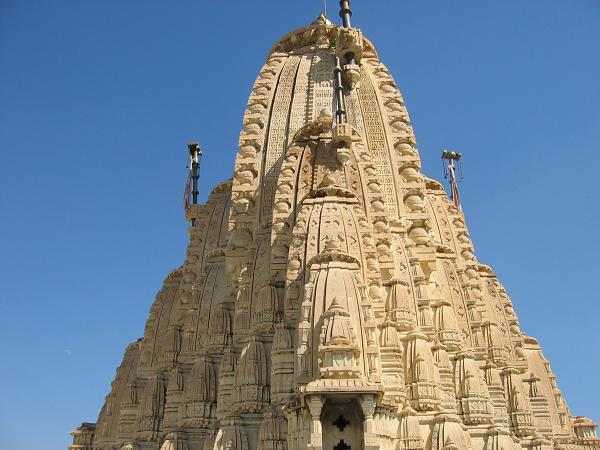
\includegraphics[width=4.8cm]{articles/Octopussy/jain.jpg}
%Un temple Jain.

Puis nous avons visite le City Palace, d'où la vue sur la ville est superbe.

%\hspace*{-0.65cm}
%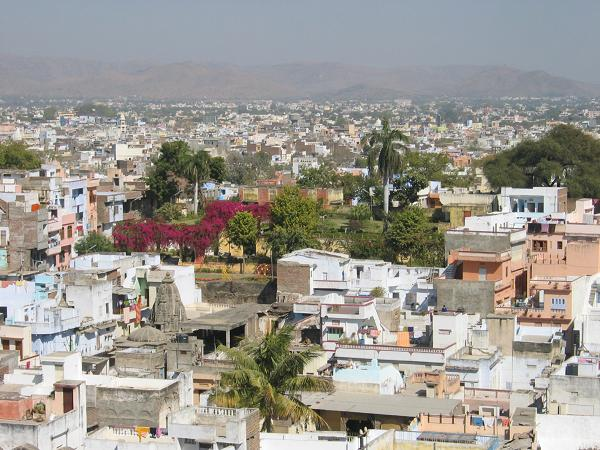
\includegraphics[width=4.8cm]{articles/Octopussy/zoomville.jpg}
%Vue sur la ville.

Udaipur est aussi connu pour avoir servi de décor au tournage du film Octopussy, James Bond. C'est un luxueux hôtel en plein milieu du lac qui est filmé.

%\hspace*{-0.65cm}
%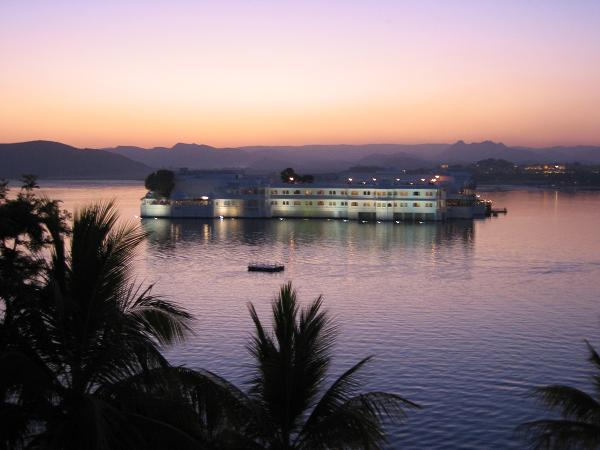
\includegraphics[width=4.8cm]{articles/Octopussy/octopussy.jpg}
%Hotel de James Bond.

Et pour finir cet article, voici un magnifique coucher de soleil sur le lac.

%\hspace*{-0.65cm}
%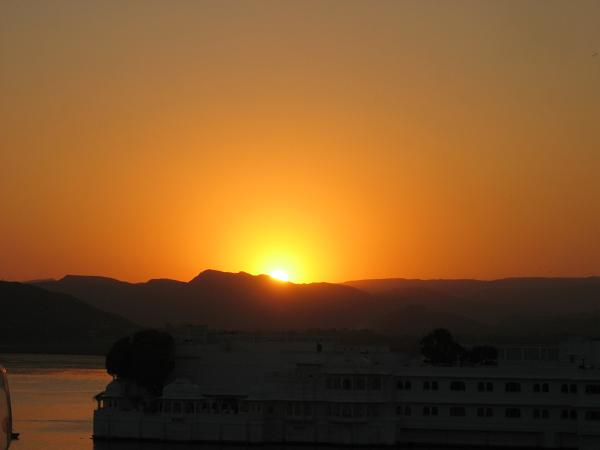
\includegraphics[width=4.8cm]{articles/Octopussy/soleil.jpg}
%Coucher de soleil.

A bientôt...

\end{multicols}

\bigskip
\textbf{\textsc{Commentaires}}

\medskip
Poun's a écrit le 16 fév. 2008 :
\begin{displayquote}
Ouah, toujours de belles images. Pas trop dur, les voyages dans les bus-couchettes sans couchettes?
Une arnaque de plus? Faites toujours attention, et faites toujours le plein d'émotions.
Les photos où tu avais l'enfant dans tes bras et toutes celles de cette page (five fingers, not the same) ont disparu. Incident technique ou censure?
Par prudence, évitez de transmettre des photos trop personnelles de vos guides et de vos contacts, et ne racontez pas sur le net les épopées pas très licites.
Mais à part ça, profitez!
A bientôt pour un nouvel épisode!
\end{displayquote}

\medskip
Jean yves a écrit le 16 fév. 2008 :
\begin{displayquote}
Je suis pas à pas votre périple,sur sur carte de l'atlas au 1/450000.Vu là dessus c'est impresionnant qu'il faille toute une nuit pour aller de Almer à Udaipur.Au Laos,nous avions ainsi pris un bus toute une nuit à travers la montagne.Ceux qui dormaient n'avaient pas vu les précipices,les villages traversés à une vitesse folle.

Question culturelle: qu'est ce qu'un temple Jain?
Nouvelles de la famille : ce soir à 10h,toujours pas de petite fille en vue à Besançon .
Bravo les photos, et le texte. c'est agréable à lire.
Juste: J'imagine que vous n'osez pas trop prendre les gens en photo. Nous non plus..c'est pourtant bien sûr ce dont on se souvient le plus après...J'ai envie de voir les Indiens.
\end{displayquote}

\medskip
Titou a écrit le 17 fév. 2008 :
\begin{displayquote}
Encore un joli article avec de magnifiques photos ! J'avoue le coup du bus sans couchettes c'était pas top comme surprise mais bon je pense que vous avez survécu sans trop de problèmes ! Profitez en toujours a fond et surtout faites gaffe à vous !
\end{displayquote}

\medskip
Annie et Jean-yves a écrit le 17 fév. 2008 :
\begin{displayquote}
EH,bien nous on va faire aussi un super voyage :
vers Besançon et vers une petite fille qui est en train de faire son arrivée sur la terre dans les heures qui viennent...On est trop contents.Bisou à tous les blogueurs Didoum,ceux qu'on connait et les autres.
\end{displayquote}

\medskip
Etienne a écrit le 17 fév. 2008 :
\begin{displayquote}
Alors, pour ceux qui n'auraient pas compris je viens d'etre tonton ce matin, j'en connais deux qui doivent etre sur un petit nuage, du cote de Besancon. Felicitation p'tite soeur et a toi aussi Jef...
Passons a la page culture : Le Jainisme
Voici le debut de la definition du Jainisme prise sur wikipedia : Le jaïnisme, ou jinisme, du sanskrit Jina «vainqueur», est une religion (en précisant que le mot religion se traduit en Inde par dharma, un mot largement polysémique qui signifie autant «foi», «religion», «vertu» que «devoir», «nature propre», «bonne action»...), un chemin spirituel qui insiste sur les concepts d'ahimsa (non-violence) et de karma et qui met l'accent sur l'ascétisme.
Pour la definition complete, <a href="http://fr.wikipedia.org/wiki/Jainisme">cliquez ici</a>.
\end{displayquote}

\medskip
Titou a écrit le 18 fév. 2008 :
\begin{displayquote}
Hey hey félicitation mon pti DUD tu es tonton ! Félicitation aussi aux parents (car c'est quand même eux qui ont fait tout le boulot :D )  et aux grands parents ! Une excellente nouvelle ça ! Ça va pouponner fort du coté de Besançon ! Bisous à tous !
\end{displayquote}

\medskip
Lydie a écrit le 18 fév. 2008 :
\begin{displayquote}
Félicitation à Etienne !
Je me répéte par rapport aux autres, mais pas mal le bus couchettes sans couchettes !!!
Les photos sont magnifiques! Vos péripéties donnent vraiment envie de faire le sac et de partir!
Profitez bien
Je pense fort à toi ma poulette !
Gros Bisous
\end{displayquote}

\medskip
Tatid a écrit le 21 fév. 2008 :
\begin{displayquote}
Félicitation nouveau tonton :-)
Ah ouais les transports, ça doit être un peu long quand même, 5h30 en bus pendant la nuit, ça doit pas être super confort quoi, mais bon, c'est le charme du pays ;-)
Je pensais à un truc, vous mettez le blog relativement à jour avec des photos et tout et tout, chapeau, pcq là-bas, je sais pas si vous trouvez facilement des cyber-café ?!
Allez, zou, j'ai d'autres photos à voir et d'autres articles à lire !
Bisous à vous deux !
\end{displayquote}

\vfill

